

\section{Method}


\newpage

\subsection{Optimal Finger Dimensions}
Material properties:
\begin{table}[h!]
	\begin{center}
		\caption{Material properties}
		\label{tab:mat_props}
	\begin{tabular}{1rrl}
		& PLA & PP & unit \\
		$E$ & {1820} &  {220} & \si{\mega\pascal} \\
		$\sigma_\text{yield}$ & {37}& {8.7} & \si{\mega\pascal} \\
		$\sigma_\text{break}$ & {37}& ? & \\
		$\epsilon_\text{yield}$ & {3.1}& {18} & \si{\percent} \\
		$\epsilon_\text{break}$ & {3.1} &  $ > 300$  & \si{\percent} \\
		$\sigma_\text{bend}$ & {78} & {13} & \si{\mega\pascal} \\
		$E_\text{bend}$ & {2490}  & {305} & \si{\mega\pascal} \\
	\end{tabular}
	\end{center}
\end{table}


When any structure would fail by breakage or plastic deformation,
the structure could be enhanced by reinforcing the location where that fault would happen.
Our interlocking structure consists of beams of two materials.
Reinforcing the beams of one material means that we reduce beams of the other material.
If we consider beams of a homogeneous width then the respective widths of the beams is subject to optimization.
The width ratio is optimal when both materials would fail under the same load:

\begin{align*}
	F_\text{PLA} &= F_\text{PP} \\
	A_\text{PLA} \times \sigma_\text{PLA} &= 	A_\text{PP} \times \sigma_\text{PP}\\
	\sigma_\text{PLA} &\approx 37 \si{\mega\pascal} \\
	\sigma_\text{PP} &\approx 8.7 \si{\mega\pascal}
\end{align*}
where $\sigma$ is the yield stress.

The optimized ratio between PLA and PP is therefore
$
A_\text{PP} / A_\text{PLA} = \sigma_\text{PLA} / \sigma_\text{PP}  \approx 4.3
$

If we choose the width of the PLA beams to be two standard lines wide, \SI{0.7}{\milli\meter}, then the PP beams should be \SI{3.0}{\milli\meter}.




The height of the beams is relatively irrelevant to the optimization.
Only when the beams are a lot higher than the layer thickness does a new failure mode come into play where the beams in the orthogonal directions shear off each other.
Given that the ultimate shear stress is approximately half the ultimate tensile stress,
this failure mode plays a role when the contact area between the beams is half the cross sectional area of a beam.
However, the width of the beams is in the order of twice the nozzle size, whereas the layer height is in the order of a quarter of the nozzle size.
If we keep the beams as high as two layers the shearing failure mode will not take effect.


\subsection{Optimal Varying Finger Width}

Let's consider a PLA finger which crosses $N$ beams, which is allowed to vary in width.
See \cref{force_distribution}.
Assuming both materials have the same stiffness $\sigma$, we can derive the optimal widths of the segments.
In case one segment would have a higher stress than the others then that one would be the weakest link, so in the optimal structure all segments have the same stress $\sigma$.

\begin{align*}
    \sigma &= \frac{F_x}{w_x h} \\
    F_x &= w_x h\sigma \\
    w &= w_x + w_{N+1-x} \\
    F_1 &= F_x + F_{N+2-x} \\
    w_1 h \sigma &= w_x h \sigma + w_{N+2-x} h \sigma \\
    w_1 &= w_x + w_{N+2-x} \\
    w_N &= w - w _1 = w_{N+1-x} - w_{N+2-x} = w_x - w_{x+1} \\
    w_x &= (N + 1 - x)  w_N \\
    w &= w_1 + w_N = N w_N  + w_N = (N+1) w_N\\
    w_N &= \frac{w}{N+1} \\
    w_x &= \frac{N + 1 - x}{N+1} w
\end{align*}

We therefore conclude that if the two materials have the same properties
the optimal fingers have a linear width change from $w$ at the base to $0$ at the tip.
However, this result doesn't extrapolate when the materials have different properties.

Given an extension $\epsilon$ of two parallel springs a and b which are connected at the ends:
\begin{align*}
    E &= \frac{\sigma}{\epsilon} \\
    \sigma &= \frac{F}{A} \\
    % F &= \sigma A = E \epsilon A \\
    % F_a &= E_a \epsilon A_a \\
    % F_b &= E_b \epsilon A_b \\
    % \frac{F_a}{F_b} &= \frac{E_a A_a}{E_b A_b} \\
    a
\end{align*}



\iffalse

\begin{figure}
	\centering
	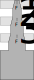
\includegraphics[height=.5\columnwidth]{sources/method/stress_distribution.pdf}
	\caption{Force distribution along a beam with varying width.}
	\label{force_distribution}
\end{figure}

\fi

